\documentclass{article}
\usepackage{proceed}

\def\argmax{\operatornamewithlimits{arg\max}}


\title{Exact Symbolic Dynamic Programming for Continuous POMDPs} 

\author{} 
          
% The author names and affiliations should appear only in the accepted paper.
%
%\author{ {\bf Harry Q.~Bovik\thanks{Footnote for author to give an 
%alternate address.}} \\  
%Computer Science Dept. \\  
%Cranberry University\\ 
%Pittsburgh, PA 15213 \\ 
%\And 
%{\bf Coauthor}  \\ 
%Affiliation          \\ 
%Address \\              
%\And 
%{\bf Coauthor}   \\ 
%Affiliation \\          
%Address    \\           
%(if needed)\\ 
%} 
 
\begin{document} 
 
\maketitle 
 
\begin{abstract} 
Decision-theoretic planning problems try to find the optimal sequence of actions for a given environment. Using continuous models in such problems is naturally closer to the real-world. Partially Observable MDPs model uncertain environments where the underlying state is not be fully observable. 

While previous work have provided solutions for discrete states and/or observations, here we define the first exact solution to both continuous state and observations. This symbolic dynamic programming approach avoids enumerating the state and observation space providing solutions for our general discrete and continuous partially observable MDP. The main contribution defines the relevant observation partitions associated with each state partition. This allows us to perform the Bellman backup operation efficiently. We address the problems in POMDP continuous planning and solutions to solve them symbolically. %To compactly represent the exact value functions Affine algebraic decision diagrams are used. 
\end{abstract} 
 
\section{Introduction} 

The following example is used throughout the paper to help better understand the definitions. 

%define example* here, just the model
\textbf{Example} \textsc{(Power Plant)}
\emph{The steam generation system of a power plant aims to provide hot steam to the steam turbine which in turn produces electricity. Feed-water is exposed to heat in the tubes leading to the water tank . Evaporating the water is performed under specific pressure and temperature inside the attached water tubes. 
Mixing water and steam pressures makes reading tank levels and temperatures very hard and uncertain. For this reason, the process is modeled using POMDP in the literature. The temperature is assumed to be a continuous variable that is not observed. Noisy observations of the temperature are used to decide on the action of closing or opening the valve.}
Most work in the literature have assumed discretization of the state and observation space ~\cite{steam2}. Here we take a continuous approach using the DC-POMDP framework.

\section{DC-POMDP Model} 
%%%% define DC-MDP
We assume familiarity with MDPs and introduce Discrete and Continuous Partially Observable MDPs as an extension to Discrete and Continuous State MDPs ~\cite{sanner_uai11}. A Discrete and Continuous partially observable MDP (DC-POMDP) is a tuple $\langle
\mathcal{S},\mathcal{A},\mathcal{O},\mathcal{T},\mathcal{R},\mathcal{Z},\gamma,h \rangle$. 
States are represented by vectors of $(\vec{d_s},\vec{x_s}) = ( d_{s_1},\ldots,d_{s_n},x_{s_1},\ldots,x_{s_m} )$ where each $d_{s_i} \in \{ 0,1 \}$ ($1 \leq i \leq n$) is a discrete boolean and each $x_{s_j} \in \mathbb{R}$ ($1 \leq j \leq m$) is a continuous variable. Actions are presented by a finite set of actions $\{ a_1, \ldots, a_p \}$. We define discrete and continuous observations by the vector $(\vec{d_o},\vec{x_o}) = ( d_{o_1},\ldots,d_{o_n},x_{o_1},\ldots,x_{o_m} )$ where each $d_{o_i} \in \{ 0,1 \}$ ($1 \leq i \leq n$) is boolean and each $x_{o_j} \in \mathcal{R}$ ($1 \leq j \leq m$) is a continuous variable. 

Three functions are required for modeling DC-POMDPs: (1) $\mathcal{T}: \mathcal{S} \times \mathcal{A} \times \mathcal{S} \rightarrow  [ 0, 1 ]$ a Markovian transition model defined as the probability of the next state given the action and previous state%$P(\vec{d}',\vec{x}'|\cdots,a)$
; (2)  $\mathcal{R}:\mathcal{S}\times\mathcal{A}\rightarrow\mathbb{R}$ a reward function which returns the immediate reward of taking an action in some state and (3) an observation function defined as $\mathcal{Z} : \mathcal{S} \times \mathcal{A} \times \mathcal{O} \rightarrow [ 0, 1 ]$  which gives the probability of an observation given the outcome of a state after executing an action.  A discount factor $\gamma, \; 0 \leq \gamma \leq 1$ is included in the model to account for future rewards in higher horizons.

%%%% forms of transition, observation and reward function
To define the transition function, we use the fact that the state variables of this POMDP can be factored into a Dynamic Bayesian Network (DBN). Not allowing synchronic arcs between the discrete and continuous variables defines their joint transition to be independent: 

{\footnotesize
\begin{equation}
P(\vec{d_s}',\vec{x_s}'|\vec{d_s},\vec{x_s},a) = 
\prod_{i=1}^n P(d_{s_i}'|\vec{d_s},\vec{x_s},a) \prod_{j=1}^m P(x_{s_j}'|\vec{d_s},\vec{d_s}',\vec{x_s},a). \nonumber 
\end{equation}}
The joint observation function can also be defined considering the direct correspondence between the state and observation variables:
{\footnotesize
\begin{equation}
P(\vec{d_o},\vec{x_o}|\vec{d_s},\vec{x_s},a) = 
\prod_{i=1}^n P(d_{o_i}|d_{s_i},a) \prod_{j=1}^m P(x_{o_j}|x_{s_j},a). \nonumber 
\end{equation}}

The \emph{binary} variables are represented using conditional probability functions (CPF) in the form of $P(d_i'|\vec{d},\vec{x},a)$. For \emph{continuous} variables
the CPF $P(x_j'|\vec{d},\vec{d'},\vec{x},a)$ is represented by \emph{piecewise
linear equations} (PLEs) that are first-order Markov and deterministic, i.e. the probabilities are encoded using the Dirac $\delta[\cdot]$ function. 

The reward function $R(\vec{d},\vec{x},a)$ is set to be any general piecewise linear  function that could facilitate pruning for space efficiency via bilinear solvers. 

For the \textsc{Power Plant} example, the temperature $t_s \in \mathbb{R}$ is modelled as the continuous state variable. Noisy observation of the temperature $t_o \in \mathbb{R}$ is used to help decide the optimal action to either open or close the pressure valve $a \in \{open,close\}$. 
For the transition probability, we use the Dirac function to model the deterministic equations. We can also define stochasticity in the transition model using boolean random variables that are sampled stochastically.  
\begin{align}
P(t_s'|\vec{t_s},a)= \delta\left[ t_s' - 
\begin{cases}
 (a=open) &: t_s + 50 \\ 
(a \neq open) &: t_s - 35 \\
\end{cases}
\right]\nonumber
\end{align}
%contribution? 
For observations we can consider discrete noise, modeled using CSEs. The probability that the observed temperature is equal to the actual temperature is $0.9$  while it indicates a higher temperature with probability of $0.1$. For the open action, observations are more disposed to noise: 

\begin{align}
P(t_o|t_s',close) = 
\begin{cases}
 \delta\left[ t_o=t_s \right] &: 0.9 \\
 \delta\left[ t_o=1.5*t_s \right] &: 0.1 \\
\end{cases}
\\
P(t_o|t_s',open) = 
\begin{cases}
 \delta\left[ t_o=1.1*t_s \right] &: 0.8 \\
 \delta\left[ t_o=1.4*t_s \right] &: 0.2 \\
\end{cases}
\end{align}
%We can extend this to consider continuous noise such as a uniform noise distribution which is more realistic in many domains. For a certain interval, the probability is a fixed number, while it is zero elsewhere. The integral of the uniform distribution should sum to one. 
%\begin{align}
%P(t_o|t_s',close) = 
%\begin{cases}
% (t_o>t_s-5) \wedge (t_o<t_s+5) &: 0.1 \\
% \neg((t_o>t_s-5) \wedge (t_o<t_s+5)) &: 0 \\
%\end{cases}
%\end{align}

The reward function can be any linear function of the state or action. Going above a threshold temperature (e.g. $T=200$) will cause an explosion in the plant when trying to close the valve which results in the negative reward of $-1000$. Staying below this temperature is safe and will produce electricity an gain the reward of $100$. The reward of an open valve is $-1$.
\begin{align}
R(t_s,a) = 
\begin{cases}
 (a=open) &: -1 \\
(a \neq open)\wedge (t_s>T) &: -1000 \\
(a \neq open)\wedge \neg(t_s>T) &: 100 \\
\end{cases}\nonumber
\end{align}
This example will try to maximize its reward using observations on the temperature. The observations recieved before closing the plant to a safe temperature are therefore critical. 

%write about policy in POMDPs
\section{DC-POMDP solution}
The DC-POMDP will choose actions in order to compute an optimal plan over time. This plan is the policy $\pi$ of the agent which depends on the history of actions and observations over a Markovian state. In the partially observable case where there is uncertainty on the states, the policy is a function over a continuous set of probability distributions over $|\mathcal{S}|$. Observations don't provide a unique state therefore a probability of the state is stored as the belief state $b$.

 At any of the horizon steps, a DC-POMDP policy $\pi(b)$ is defined as the iterative plan on executing an action and observing all probable outcomes of the set of observations from the $(h-1)$-step. The belief state is updated after this according to the Bayes rule: $\sum_{d_s}\int_{x_s} b(xd_s)T(xd'_s,xd_s,a)Z(xd'_s,xd_o,a)$  where for simiplicity we use ($xd_s = x_s,d_s$) and ($xd_o=x_o,d_o$).
The optimal policy is defined over the belief state as the sum of the expected discounted rewards over horizon $h$ starting with belief $b_0$.
\begin{equation}
V^h_{\Pi^*}(\vec{b}) = E_{\pi^*} \left[ \sum_{h=0}^{H} \gamma^t \cdot r_h \Big| \vec{b}_0 = \vec{b} \right]\nonumber
\end{equation}
The next section provides the mathematics required to solve this equation in DC-POMDPs.
%%%%%%%%%%%%%%%%%%%%%%%%%%%%%%%%%%%%%%%%%%%%%%%%%%%%%%%%%%%%%%%%%%%%%%%%
% Figure 1 - policy tree
\begin{figure}[t!]
%\vspace{-1mm}
\begin{center}
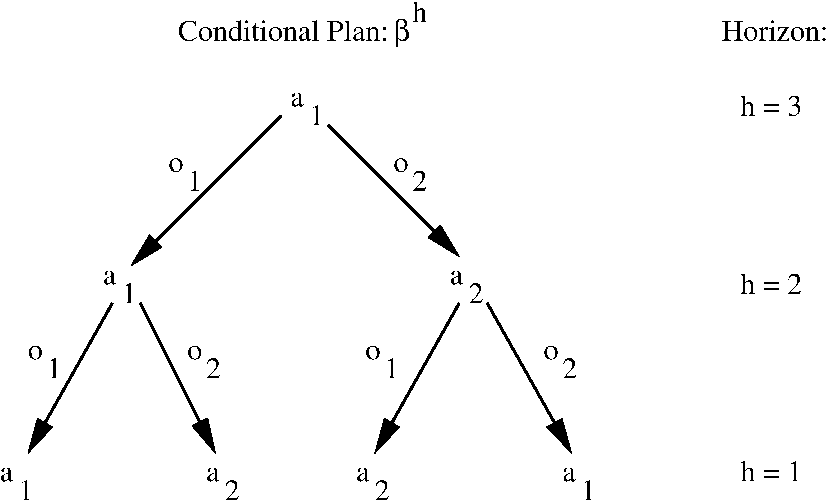
\includegraphics[height=4cm]{cond_plan2}
\end{center}
\vspace{-2mm}
\caption{\footnotesize Example conditional plan $\beta^h$ for discrete observations.}
\label{fig:cond_plan}
\vspace{-1mm}
\end{figure}
%%%%%%%%%%%%%%%%%%%%%%%%%%%%%%%%%%%%%%%%%%%%%%%%%%%%%%%%%%%%%%%%%%%%%%%%

\subsection{Value Iteration solution} 
%solutions with belief
Solving the value function for the optimal policy is performed using Dynamic programming algorithms such as value iteration. 
The decision at each time step is to pick an action based on past actions and observations. The possible set of conditional plans $\beta^h$ correspond to a decision tree. Figure 1 shows the decision tree for the simple case of three horizons with discrete observations. It represents a conditional plan consisting of an action and two possible observation strategies. For continuous observations, conditional plans are decision trees with infinitely many branches. In our solution we show that instead of a policy tree with infinite branches, we can create partitions based on relevant observation values, resulting in a policy tree similar to that of figure 1. We prove that a finer grain partitioning of the observation space has the same properties of the minimal partition set. From here on we assume this finite set of observation partitioning as $\mathcal{O}$.

The value iteration algorithm finds the optimal value for each horizon starting with an initial belief. Although the number of belief states is infinite, the optimal value function for $h$ is proven to be a piecewise linear and convex function of the belief state \cite{smallwoodSondik}. The optimal value function is the maximum value over a finite set of alpha vectors  $\alpha^h_i$:%that define the hyperplanes:
\begin{equation}
V^h_{\Pi^*}(\vec{b}) = \max_{\alpha^h_i \in \Gamma^h} \alpha^h_i \cdot \vec{b}
\end{equation}
where the belief states $\vec{b}$ and each $\alpha^h_i \in \Gamma^h$ are of dimension $|\mathcal{S}|$. At each of the $h$-steps the value function is parameterized by the set of  $\alpha$-vectors that partition the belief state. 
At a particular belief point, we can compute the next value function: 
\begin{align*}
V^{h+1}(b) = \max_a \left( b \cdot r_a + \gamma \sum_o p(xd_o|a,b)V^h(b|xd_o,a)\right)\nonumber
\end{align*}
Replacing the previous iteration value with (3) and also updating the belief after executing action $a$ and observing $xd_o$ results in the following equation: 
\begin{align*}
V^{h+1}(b) = \max_a \left( b \cdot r_a + 
\gamma \sum_o \max_{\langle g^h_{a,o,j} \rangle_j}  b \cdot g^h_{a,o,j} \right)\nonumber
\end{align*}
where $r_a = r(x_s,d_s,a)$ and  
\begin{align}
g^h_{a,o,j} =  \int_{x_{s'}} \sum_{d_{s'}} p(xd_o|xd'_s,a)p(xd'_s|xd_s,a) \alpha^h_j(xd'_s)
\end{align}

Calculating all possible ways of building the value function independent of a certain belief state can also define the optimal value function. To derive the $\Gamma$-set of all possible $\alpha$-vectors for each horizon, we use the value iteration algorithm from (Monahan)~\cite{monahan82}. 
Initializing  $\alpha^0_1 = \vec{0}$ and $\Gamma^0 = \{ \alpha^0_1 \}$, $\Gamma^h$ is obtained from $\Gamma^{h-1}$ using the backup operation defined in (4):\footnote{The $\textrm{\large $\boxplus$}$ of sets is defined as 
$\textrm{\large $\boxplus$}_{j \in \{ 1,\ldots, n \} } S_j = S_1 \textrm{\large $\boxplus$} \cdots \textrm{\large $\boxplus$} S_n$ where the pairwise cross-sum $P 
\textrm{\large $\boxplus$} Q = \{ \vec{p} + \vec{q} | \vec{p} \in P, \vec{q} \in Q \}$.}
\begin{align}
\Gamma^{h}_a   &= r_a + \gamma \textrm{\large $\boxplus$}_{o \in \mathcal{O}} \left\{ g^h_{a,o,j}(\cdot) \right\}_j ;  \forall \alpha^{h-1}_{j} \in \Gamma^{h-1}  \\
\Gamma^h  &= \bigcup_a \Gamma^h_a 
\end{align}
Each action-dependent $\Gamma$ sums over the possible set of $g^h_{a,o,j}(\cdot)$ given a relevant observation partition $(xd_o)$ and for all $\alpha^{h-1}_{j} \in \Gamma^{h-1} $. The value $g^h_{a,o,j}(\cdot)$ is computed by summing over all states given the probability functions and previous $\alpha$-vectors.  
For each horizon, the optimal $\alpha$-vector is obtained from the maximum over all $\alpha$-vectors: 
\begin{align}
\alpha^* = \argmax_{\alpha^h_i \in \Gamma^h} \alpha^h_i \cdot b \nonumber
\end{align}

For discrete observations, the cross-sum operation takes the set of $\alpha$ -vectors for each observation and produces a sum over vectors that depends on the number of previous iteration vectors. Thus the $\alpha$-vector set grows exponentially in the number of observations, i.e., $|\Gamma^{h}| = |\mathcal{A}|
|\Gamma^{h-1}|^{|\mathcal{O}|}$ during the cross-sum operation. For this reason even for a small number of discrete observations, tractable solutions may be hard to define. Here we do not restrict our observations to discrete ones, but extend it to a fully continuous approach where continuous observations and states are allowed in the DC-POMDP. We use the number of  observation partitions $|\mathcal{O}|$ as the branching factor in the policy tree. We present the symbolic value iteration algorithm and approaches to solving this problem in the following section. 

\section{Symbolic Dynamic Programming} 
Dynamic programming provides exact solutions to POMDP problems for small domains. As the domain grows, fully enumerating the state, action and observation space leads to intractable solutions even for low horizons. Avoiding this enumeration often requires approximating the solutions. We claim an exact solution using symbolic dynamic programming. The SDP solution for fully observable domains has been presented in \cite{sanner_uai11} %using piecewise constant functions
Our symbolic algorithm deals with continuous observations and states by generating the relevant observation partition at every time step and performing the backup operation using $\alpha$-vectors. We define the requirements to implement the value iteration for DC-POMDP. 

\subsection{Case Representation and Extended ADDs}
% operations, max, restrict, substitute
%overview + example plant
The \textsc{Power Plant} example represented all functions using the case structure which can be generally defined as:
{%\footnotesize 
\begin{align}
f = 
\begin{cases}
  \phi_1: & f_1 \\ 
 \vdots&\vdots\\ 
  \phi_k: & f_k \\ 
\end{cases} \nonumber
\end{align}
}
Where $\phi_i$ are disjoint logical formulae defined over the state $(\vec{d},\vec{x})$ with logical ($\land,\lor,\neg$) combinations of boolean variables and inequalities ($\geq,>,\leq,<$) over continuous variables.  
The $f_i$ are function definitions either linear or quadratic in the continuous parameters. 

For \emph{unary operations} such as scalar multiplication $c\cdot f$ (for some constant $c \in \mathbb{R}$) or negation $-f$ on case statements is simply to apply the operation on each case partition $f_i$ ($1 \leq i \leq k$). 

A \emph{binary operation} on two case statements, takes the cross-product of the logical partitions of each case statement and performs the corresponding operation on the resulting paired partitions.  The cross-sum $\oplus$ of two cases is defined as the following:

{\footnotesize 
\begin{center}
\begin{tabular}{r c c c l}
&
\hspace{-6mm} 
  $\begin{cases}
    \phi_1: & f_1 \\ 
    \phi_2: & f_2 \\ 
  \end{cases}$
$\oplus$
&
\hspace{-4mm}
  $\begin{cases}
    \psi_1: & g_1 \\ 
    \psi_2: & g_2 \\ 
  \end{cases}$
&
\hspace{-2mm} 
$ = $
&
\hspace{-2mm}
  $\begin{cases}
  \phi_1 \wedge \psi_1: & f_1 + g_1 \\ 
  \phi_1 \wedge \psi_2: & f_1 + g_2 \\ 
  \phi_2 \wedge \psi_1: & f_2 + g_1 \\ 
  \phi_2 \wedge \psi_2: & f_2 + g_2 \\ 
  \end{cases}$
\end{tabular}
\end{center}
}
\normalsize

Likewise $\ominus$ and $\otimes$ are defined by subtracting or multiplying partition values.  Inconsistent partitions can be discarded when they are irrelevant to the function value.
% Do I need maximization for VI? 
%%%%%%%%%%%%%%%%%%%%%%%%%%%%%%%%%%%%%%%%%%%%%%%%%%%%%%%%%%%%%%%%%%%%%%%%%%
%Define V^2 here?
\begin{figure}[t]
\begin{center}
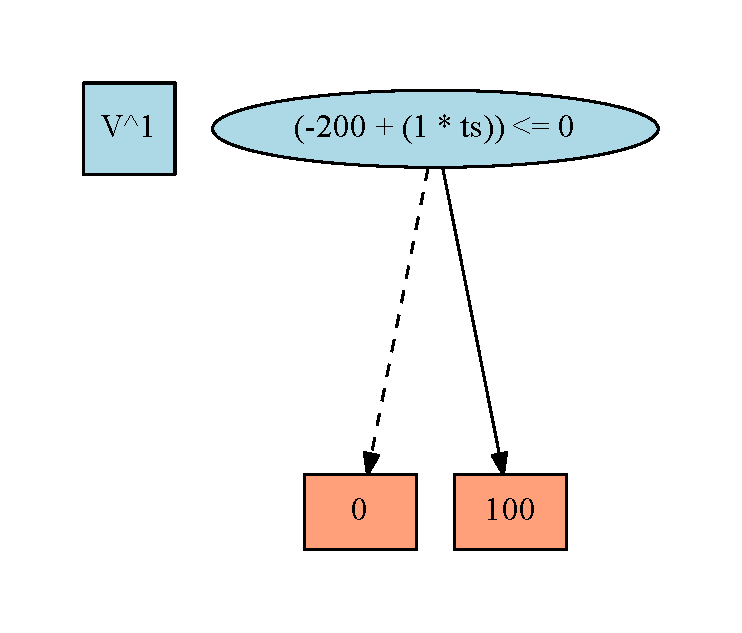
\includegraphics[width=0.4\textwidth]{v1.pdf}
\end{center}
\vspace{-3mm}
\caption{%\footnotesize 
The optimal value function for \textsc{Power Plant}
as a decision diagram: 
the \emph{true} branch is solid, the \emph{false}
branch is dashed.} 
\end{figure}
%%%%%%%%%%%%%%%%%%%%%%%%%%%%%%%%%%%%%%%%%%%%%%%%%%%%%%%%%%%%%%%%%%%%%%%%%%
%xadd representation
The data structure of \emph{extended ADD} (XADD)~\cite{sanner_uai11} is used to support
case statements and the required operations.  Here we use continuous SDP for both states and observations in DC-POMDPs. The value functions and $\alpha$-vectors partition into states of equal value, both of which can be represented using XADDs. For increasing efficiency linear constraint feasibility checkers such as LP solvers allow pruning unreachable paths in the XADD.

%%%%%%%%%%%%%%%%%%%%%%%%%%%%%%%%%%%%%%%%%%%%%%%%%%%%%%%%%%%%%%%%%
\incmargin{.5em}
\linesnumbered
\begin{algorithm}[t!]
\vspace{-.5mm}
\dontprintsemicolon
\SetKwFunction{substitute}{Substitute}

\Begin
{
	$\textsc{O}:=\emptyset$ \;	
	\For {all $\alpha_j^{'h}$ in  $\Gamma^h$}    
	{
    	\emph{Relevant state partitions $\phi_j^{'h}$ of $\alpha_j^{'h}$}\\   
   	 	\For {all $xd'_{s_i}$ in $\phi_j^{'h}$}
   		 {
    		$\phi_{xd_s} := $ $\phi\{xd_{s_i}\setminus xd_{o_i}$\}\ \;
    		$\alpha_{j,o_i}^{h} := P(xd_{o_i}|xd'_{s_i},a) * \phi_{xd_s}$;\
    	}
    	$\textsc{O}^h := \oplus \alpha_{j,o}^{'h}$\;
    }
    \Return{$\textsc{O}^{h}$} \;
}
\caption{\footnotesize \texttt{GenRelObs}($\Gamma^h,a$) $\longrightarrow$ $\textsc{O}^{h}$ }
\vspace{-1mm}
\end{algorithm}
\decmargin{.5em}
%%%%%%%%%%%%%%%%%%%%%%%%%%%%%%%%%%%%%%%%%%%%%%%%%%%%%%%%%%%%%%%%%
%%%%%%%%%%%%%%%%%%%%%%%%%%%%%%%%%%%%%%%%%%%%%%%%%%%%%%%%%%%%%%%%%
\incmargin{.5em}
\linesnumbered
\begin{algorithm}[t!]
\vspace{-.5mm}
\dontprintsemicolon
\Begin{
   
    \emph{// Continuous regression, marginal integration}\\
    \For {all $x_{s_j}'$ in $\alpha_{j,o}^{'h}$}
    {
         $G_a^h := \int \textsc{O}^{h} \otimes P(x_{s_j}'|\vec{d_s},\vec{d_s}',\vec{x_s},a) \, d_{x_{s_j}'}$\;
    }
    \emph{// Discrete regression, marginal summation}\\
    \For {all $d_{s_i}'$ in $\alpha_{j,o}^{'h}$}
    {
         $G_a^h := \left[ G_a^h \otimes P(d_{s_i}'|\vec{d_s},\vec{x_s},a) \right]|_{d_{s_i}' = 1}$\\
         \hspace{8mm} $\oplus \left[ G_a^h \otimes P(d_{s_i}'|\vec{d_s},\vec{x_s},a) \right]|_{d_{s_i}'= 0}$\;
    }
    \Return{$G_a^h$} \;
}
\caption{\footnotesize \texttt{Backup}($\alpha_{j,o}^{'h},a,$) $\longrightarrow$ $G_a^h$ \label{alg:regress}}
\vspace{-1mm}
\end{algorithm}
\decmargin{.5em}
%%%%%%%%%%%%%%%%%%%%%%%%%%%%%%%%%%%%%%%%%%%%%%%%%%%%%%%%%%%%%%%%%

%%%%%%%%%%%%%%%%%%%%%%%%%%%%%%%%%%%%%%%%%%%%%%%%%%%%%%%%%%%%%%%%%
%\incmargin{.5em}
%\linesnumbered
%\begin{algorithm}[t!]
%\vspace{-.5mm}
%\dontprintsemicolon
%\Begin{
%	\emph{any function f has $i$ partitions like $\phi_i:f_i$}\;	
%	\emph{compute UB and LB from $\phi_i$ using constraints on $var$}\;
%    $I=$ \emph{ any $var$-independent $\phi_i$} \;
%    $F = $ \emph{differentiate $f_i$}\;
%    $F = I \otimes [F(UB) - F(LB)]$\;
%    \Return{$F$} \;
%}
%\caption{\footnotesize \texttt{VE}($var,f$) $\longrightarrow$ $F$ }
%\vspace{-1mm}
%\end{algorithm}
%\decmargin{.5em}
%%%%%%%%%%%%%%%%%%%%%%%%%%%%%%%%%%%%%%%%%%%%%%%%%%%%%%%%%%%%%%%%%
\subsection{Continuous Observation Space} 
%progression definition
The main operations required for value iteration in DC-POMDP is generating relevant observations and perform the bellman backup operation. 
%Progression is the inverse of regression. The \emph{regression} of a formula $\psi$ through an action $a$ is a formula $\psi'$ that holds prior to $a$ being performed iff $\psi$ holds after $a$. \emph{Progression} takes a formula $\psi$ and an action $o$ and represents the formula $\psi'$ that would hold after action $o$ is performed in a situation satisfying $\psi$.

The \texttt{GenerateRelObs} algorithm defines the operation of generating relevant observation partitions. Starting with an empty set of relevant observation partitions $\textsc{O}^{h}$, the algorithm iterates through all possible $\alpha$-vectors of the previous horizon. For each of the vectors, we use the state partitions of that $\alpha$-vector where the logical formulas $\phi_j^{'h}$ of the cases are defined as the state partitions. 

Lines 5--7 iterate on all the state variables (both discrete and continuous) of a certain state partition $\phi_j^{'h}$. In line 6 the state variables are substituted with the observation variables based on the observation model provided. In the next line the probability attached to the observation given this state and the input action is multiplied in the relevant observation partition to produce a single case partition with a logical formula depending on observations and a probability based on the observation model.
In other words, lines 5-7 take a state partition and return an observation partition that is only relevant to the states according to $\mathcal{Z} : \mathcal{S} \times \mathcal{A} \times \mathcal{O} \rightarrow [ 0, 1 ]$. 
Finally for every specific $\alpha$-vector, the relevant observation partitions are added to the set of all relevant observations $\textsc{O}^{h}$ regardless of the vector they came from. The operator $\oplus$ only performs the operation on the logical formulas $\phi_i$ of the case partitions,without actually adding the function values. 

To illustrate the algorithm with an example, we assume a discrete %and continuous 
noise distribution model such as (1). We explain each step of the algorithm using the \texttt{Power Plant} example. Assume that after $h=1$ the set of $\alpha$-vectors are defined as:
\begin{align}
\alpha_1^1(s) &= 
\begin{cases}
 (t_s>200) &: -1000 \\
\neg(t_s>200) &: 100 \\
\end{cases}
\alpha_2^1(s) &= \top &: -1
\end{align}
The relevant state partition only considers the logical formulas: $\{t_s>200, t_s<200\}$. For horizon $h=2$ and specific action $close$ we derive the relevant set of observations for both $\alpha_1^1$ and $\alpha_2^1$. The discrete noise observation model (1) is used for the substitution step where $t_o$ is substituted with $t_s$ most of the times(i.e, with probability 0.9) and $2/3t_o=t_s$ with probability of 0.1. By replacing these inside the state partitions, the relevant observation partitions are formed: 
\begin{align*}
\begin{tabular}{r c c c l}
&
\hspace{-6mm} 
$\alpha_1^1(t_s'>200) $&= 
$\begin{cases}
  t_o>200 \\
   t_o>300  \\
 \end{cases}$
 \\
 &
\hspace{-6mm} 
$\alpha_1^1(t_s'<200) $ &= 
$\begin{cases}
 t_o<200 \\
 t_o<300 \\
\end{cases}$
&
\hspace{-4mm} 
$\alpha_2^1(t_s'>200) = \top$
\end{tabular}
\end{align*}
The probabilities of each partition is then multiplied according to the noise model and the two vectors are added to the relevant observation set $\textsc{O}^{h}$. In our example $\alpha_2^1$ will leave no effect in the final set proposing a partitioning on the observation space depending on the relevant state space partition. The probability of receiving observations between ($200,300$),given that the next state has high temperatures (higher than $200$) is $0.9$. We name the three partitions as the observation partitions of $O_1,O_2,O_3$:

\begin{align*}
O_1:P(200<t_o<300 |t_s',close) = 
\begin{cases}
 % 2*t_o>200 &: 0.7 \\
 %2/3*t_o>200 &: 0.3 \\
% 2*t_o<200 &: 0.7 \\
 %2/3*t_o<200 &: 0.3 \\
  t_s'>200 &: 0.9 \\
\neg(t_s'>200) &: 0.1 \\
 \end{cases}
 \\
 \hspace{-4mm} 
O_2:P(t_o>300|t_s',close) = 
\begin{cases}
 t_s'>200 &: 0.1 \\
 \neg(t_s'>200) &: 0.0 \\
 \end{cases}
\\
\hspace{-4mm} 
O_3:P(t_o<200|t_s',close) = 
\begin{cases}
 t_s'<200 &: 0.9 \\
 \neg(t_s'>200) &: 0.0 \\
\end{cases}
\end{align*}
%For continuous noise models such as (2) lines 8--11 is used. To progress a continuous observation from a continuous next state according to noise, we use a symbolic variable elimination inference approach %mentioned in \cite{sve}. 
%To compute  $\int_{x_1=-\infty}^{\infty} f \, dx_1$ for some case-statement function $f$ we define the the following: 
%\vspace{-2mm}
%{\footnotesize
%\begin{equation}
%\int_{x_1=-\infty}^{\infty} \sum_i \mathbb{I}[\phi_i] \cdot f_i \, dx_1 \; = \; \sum_i \int_{x_1=-\infty}^{\infty} \mathbb{I}[\phi_i] \cdot f_i \, dx_1 \nonumber
%\vspace{-1mm}
%\end{equation}
%}
%where $\mathbb{I}[\cdot]$ is an indicator function taking value 1 when its argument is true, 0 when it is false.  We can compute the integrals separately for each case partition and $\sum$ the results using the case sum $\oplus$.
%
%For any single case partition, the integral is computed by a number of steps defined in the VE algorithm. For each case in $\alpha^h_j$ and for each state variable that is to be eliminated $x_{s_i}$, we perform a step of the VE algorithm. First the upper and lower bounds of the logical formulas of $\phi_{i,j} \in \alpha^h_j$ are computed. Any value less than ($<$ , $\leq$) of $x_{s_i}$ is considered a lower bound (LB) and any value greater is an upper bound. For the noise model of (2) and according to the first case statement of $\alpha^1_1$ the LB and UB are defined as below: $LB := max \left\langle 200,t_o - 5 \right\rangle , UB:=\left\langle t_o + 5\right\rangle$
%
%If a certain $\phi_{i,j}$ does not constrain on $x_{s_i}$, then this is added to an indicator function  $\mathbb{I}$. After evaluating the integral of the function $f_{i,j}$, the result is obtained by substituting the bounds and multiplying by the independent constraints. 
%\vspace{-1mm}
%\begin{equation*}
%\mathbb{I}[0.1] \int_{x_{s_i}=\mathit{LB}}^{\mathit{UB}} (-1000) \, dx_{s_i} = 0.1  \left[ -1000 * x_{s_i} \bigg|_{x_{s_i}=\mathit{LB}}^{x_1=\mathit{UB}} \right]
%\end{equation*}
%
%The case statement of the observation probability is defined over all partitions of $\alpha^h_j$: 
%\begin{align*}
%P(t_o|t_s'>200,close) &=
%\begin{cases}
% % 2*t_o>200 &: 0.7 \\
% %2/3*t_o>200 &: 0.3 \\
%% 2*t_o<200 &: 0.7 \\
% %2/3*t_o<200 &: 0.3 \\
%  t_o>205 &: -10,000 \\
% t_o<205 &: -1195 - 1000*t_o \\
% \end{cases}
% \\
% P(t_o|t_s'<200,close) &= 
%\begin{cases}
% t_o<195 &: 305 - 100*t_o \\
% t_o>195 &: 1000 \\
%\end{cases}
%\end{align*}

% regression in value iteration
Backup of an observation-weighted transition function where the weights are determined according to the relevant observation partitions is explained in the \texttt{Regress}. It is composed of two main parts:

\emph{Boolean restriction} is defined in lines 5--8 where $f|_{b=v}$ restricts a boolean variable $b$ occurring in $f$ to values $v \in \{ 0,1 \}$. This can be done by simply appending $b=v$ to each case partition (logical $\wedge$ of $b=v$ and the logical first-order formulas of $f$). 

\emph{Continuous regression} $\int f(x_{s_j}') \otimes P(x_{s_j}'|\cdots) dx_{s_j}'$ in line 3--4 has the form $\delta[x_{s_j}' - h(\vec{z})]$ for the probability over the next state, where $h(\vec{z})$ is a case statement and $\vec{z}$ does not contain
$x_{s_j}'$.  A symbolic substitution is defined for this integration such that any occurrence of $x_{s_j}'$ in $f(x_{s_j}')$ is substituted with $h(\vec{z})$: 
$\int f(x_{s_j}') \otimes \delta[x_{s_j}' - h(\vec{z})] dx_{s_j}' = f(x'_j) \{ x_{s_j}' / h(\vec{z}) \}$

In our example the $\alpha$-vectors of the previous horizon use the transition probability to produce the substituted case partitions for all continuous state variables $x'_{s_i}$: 

\begin{align}
\hspace{-4mm} 
G_{close}^2= 
\begin{cases}
(t_s'>235) &: -1000 \\
\neg(t_s'>235) &: 100 \\
\end{cases}
\end{align}
\begin{align*}
G_{open}^2=  \top &: -1
\end{align*}



\subsection{Value iteration for DC-POMDPs} 

%%%%%%%%%%%%%%%%%%%%%%%%%%%%%%%%%%%%%%%%%%%%%%%%%%%%%%%%%%%%%%%%%%%%%%%%
\incmargin{.5em}
\linesnumbered
\begin{algorithm}[t!]
\vspace{-.5mm}
\dontprintsemicolon
\SetKwFunction{backup}{Backup}
\SetKwFunction{genObs}{GenRelObs}
\SetKwFunction{prune}{Prune}
\SetKwFunction{remapWithPrimes}{Prime}
\Begin
{
   $V^0:=0, h:=0$\;
   \While{$h < H$}
   {
       $h:=h+1, \Gamma^h :=\emptyset$\;
       \ForEach {$a \in A$}
       {
			$\Gamma_{a}^h :=\emptyset$ \;       		
       		$\textsc{O}^{h-1} \,:=\,$ \genObs{$\Gamma^{h-1},a$}\;
       		 \ForEach {$o_i \in \textsc{O}^{h-1}$}
       		 {
				\ForEach {$\alpha_j^{h-1} \in \Gamma^{h-1}$}
       			{
   	 		  		$\alpha_j^{h'}=$ \remapWithPrimes{$\alpha_j^{h}$} \;
   	 		  		\emph{// $\forall$ $d_i \to d_i'$ and $\forall x_i \to x_i'$} \; 
   	 		    	$\Gamma_{a,o_i,j}^h \,:=\, o_i \otimes$ \backup{$\alpha_j^{h'},a$}\;
       	      	}
       	      	$\Gamma_{a,o}^h\,:=\,\textrm{\large $\boxplus$} \Gamma_{a,o_i}^h$\;
       	     }
           $\Gamma_a^{h} \,:=\,R_a \oplus \gamma \cdot \Gamma_{a,o}^h$\;
            $\Gamma^{h} \,:=\, \Gamma^{h} \cup \Gamma_a^{h}$\;
        }  
        	%monahan's pruning first generates all vectors, then prunes
              $V^{h} \,:=\, $\prune{$\Gamma^h$} \;
              $\pi^{*,h} \,:=\, \argmax_{a} \, \Gamma_a^{h}$\;

       \If{$V^h = V^{h-1}$}
           {break $\,$ \emph{// Terminate if early convergence}\;}
   }
     \Return{$(V^h,\pi^{*,h})$} \;
}
\caption{\footnotesize \texttt{VI}(DC-POMDP, $H$) $\longrightarrow$ $(V^h,\pi^{*,h})$ \label{alg:vi}}
\vspace{-1mm}
\end{algorithm}
\decmargin{.5em}
%%%%%%%%%%%%%%%%%%%%%%%%%%%%%%%%%%%%%%%%%%%%%%%%%%%%%%%%%%%%%%%%%
%overview + example plant
Having defined the two main algorithms to produce the relevant observation partitions and the backup operation, we now explain the value iteration algorithm as defined in \texttt{VI} for DC-POMDPs. Each step of the algorithm is explained using the \textsc{Power plant} example for the first three horizons.

For $h=0$, $V^0$ is given in line 2.  For $h=1$ we choose an action, for example $close$ to start with. The $\alpha$-vector set from $h=0$ is empty so line 7 of generating the relevant observation partitions is empty. Also priming the vectors and obtaining the product of relevant observations and the backup is an empty set. In line 15 the reward $R(s,close)$ is added to obtain $\alpha^1_{1,close}$ as defined by (8). The same operation is repeated for the $open$ action where $R(s,open)=-1$. Line 16 defines the final $\Gamma$-set: 
$\Gamma^1 = \{ \alpha^1_{1,open}, \alpha^1_{1,close} \}$.

For $h=2$, for each of the discrete actions, first we generate the relevant set of observations. This has been done for the $close$ action in the previous section. Next for each of the relevant partitions and both $\alpha$-vectors of the previous $\Gamma$ set lines 8--15 are executed. 

Line 10 will substitute prime values for all state variables. Line 12 produces the backup $\alpha$-vector and multiplies it by the weight derived from the relevant observation partition. For each observation, two vectors are formed for each corresponding $\alpha$-vector. For example line 12 for observations $O_2,O_3$ and $\alpha_1^1,\alpha_2^1$ is defined as:

\begin{align*}
%\begin{cases}
%\Gamma_{close,O_1,1}^2= 
%\begin{cases}
%(200<t_o<300) \wedge (t_s'>235) &: -900 \\
%(200<t_o<300)\wedge (200<t_s'<235) &: 90 \\
%(200<t_o<300) \wedge (t_s'<200) &: -10 \\
%\end{cases}
%\\
%\Gamma_{close,O_1,2}^2= 
%\begin{cases}
%(200<t_o<300) \wedge (t_s'>200) &: -0.9 \\
%(200<t_o<300) \wedge (t_s'<200) &: -0.1 \\
%\end{cases}
%\end{cases}
%\\
\begin{cases}
\Gamma_{close,O_2,1}^2= 
\begin{cases}
(t_o>300) \wedge (t_s'>235) &: -100 \\
(t_o>300)\wedge (200<t_s'<235) &: 10 \\
(t_o>300) \wedge (t_s'<200) &: 0 \\
\end{cases}
\\
\Gamma_{close,O_2,2}^2= 
\begin{cases}
(t_o>300)\wedge (t_s'>200) &: -0.1 \\
(t_o>300) \wedge (t_s'<200) &: 0 \\
\end{cases}
\end{cases}
\\
\begin{cases}
\Gamma_{close,O_3,1}^2= 
\begin{cases}
(t_o<200) \wedge (t_s'>235) &: -900 \\
(t_o<200)\wedge (200<t_s'<235) &: 90 \\
(t_o<200) \wedge (t_s'<200) &: 0 \\
\end{cases}
\\
\Gamma_{close,O_3,2}^2= 
\begin{cases}
(t_o<200) \wedge (t_s'>200) &: -0.9 \\
(t_o<200)\wedge (t_s'<200) &: 0 \\
\end{cases}
\end{cases}
\end{align*}

Next in line 13 we have to take the cross-sum of the two sets which takes every possible combination of observations according to the $\alpha$-vectors. This means for $O_2 \textrm{\large $\boxplus$} O_3$ we have the following vectors: 

\begin{align*}
\begin{cases}
\begin{cases}
(t_s'>235) &: -1000 \\
(200<t_s'<235) &: 100 \\
(t_s'<200) &: 0 \\
\end{cases}
\\
\begin{cases}
(t_s'>235) &: -100.9 \\
(<200<t_s'<235) &: 9.1 \\
(t_s'<200) &: 0 \\
\end{cases}
\\
\begin{cases}
 (t_s'>235) &: -900 \\
 (200<t_s'<235) &: 89.9 \\
 (t_s'<200) &: 0 \\
\end{cases}
\\
\begin{cases}
(t_s'>200) &: -1 \\
(t_s'<200) &: 0 \\
\end{cases}
\end{cases}
\end{align*}

Where the observation partitions ($t_o>300 , t_o<200$) are inconsistent and therefore omitted from the result. These 4 vectors are added with the two vectors from $\Gamma_{close,O_1}^2$ to get $2^3$ different vectors. All 8 vectors are multiplied by the discount $\gamma$ and added with the reward in line 14 where the addition is an augmented $\oplus$ for adding each vector with the reward function. 
% need to add this?
The same operation is performed for the $open$ action and 8 different vectors are formed here too. In line 15 the $\Gamma$ set for each action are added to the set of $\Gamma^h$ to build all the vectors (16 in total) for the next horizon. 

In line 16 this final set is using in the \texttt{Prune} algorithm. For all $\alpha$-vectors in the current $\Gamma$-set first an LP-solver is used to prune any inconsistency in the branches of this vector. Next a pairwise dominance test is performed where for all $j,k$: 
$\alpha_j(\vec{s}) \geq \alpha_k(\vec{s})$
The result of this pairwise test is a dominant $\alpha$-vector which is added to the set of $V^h$. As an example from the set $\Gamma^2_{open,close}$ the two $\alpha$-vectors of $\alpha_{1,open}(\vec{s}) \geq \alpha_{1,close}(\vec{s})$ are tested: 
\begin{equation*}
(t_s>200) \wedge (200<t_o<300) \geq (t_s>150) \wedge (220<t_o<280)
\end{equation*}
The second $\alpha$-vector is omitted from the overall answer since it is dominated by $\alpha_{1,open}$.
%%%%%%%%%%%%%%%%%%%%%%%%%%%%%%%%%%%%%%%%%%%%%%%%%%%%%%%%%%%%%%%%%%%%%%%%
\incmargin{.5em}
\linesnumbered
\begin{algorithm}[t!]
\vspace{-.5mm}
\SetKwFunction{lpsolve}{LP-Solve}
\SetKwFunction{dominancy}{Dominance}
\Begin
{
   		$V^h :=0$ \;
       \ForEach {$\alpha_j^h \in \Gamma^h$}
       {
           $\alpha_j^h \,:=\,$\lpsolve{$\alpha_j^h$} \;
           \ForEach {$\alpha_k^h \in \Gamma^h$}
           {
				\If {$j \neq k$}  
				{         
           			$V^h \,:=\,\oplus$ \dominancy{$\alpha_j^h,\alpha_k^h$} \; 
           		}  
           	}
       }
     \Return{$(V^h)$} \;
}
\caption{\footnotesize \texttt{Prune}($\Gamma^h$) $\longrightarrow$ $(V^h)$ }
\vspace{-1mm}
\end{algorithm}
\decmargin{.5em}
%%%%%%%%%%%%%%%%%%%%%%%%%%%%%%%%%%%%%%%%%%%%%%%%%%%%%%%%%%%%%%%%%
\section{Empirical Results}

\section{Related Work}  

\section{Conclusion}

 
 
\subsubsection*{References} 
\bibliography{dcpomdp}
\bibliographystyle{plain}


 
\end{document} 



